In the course of this project I developed open-source software tools and
analysis scripts. The \texttt{iatv} package provides an API to programmatically
scrape the Internet Archive's TV News Archive (TVNA). \texttt{Metacorps}
provides methods for searching for potential metaphor, loading all potential
metaphor into a database, collaborative coding the potential metaphor in a 
browser-based app, and a data analysis pipeline for the coded metaphors. 

\subsection{iatv: open source tool for TVNA scraping}
\label{subsec:iatv}

To access the data on the TVNA, I developed a new, open-source 
software tool in the Python programming language called \textit{iatv}
\cite{Turner2016}. More details can be found on the GitHub repository page
at \url{http://github.com/mtpain/iatv}. But as a brief example, here is
how one would download all transcripts and the associated metadata from
all shows aired on Fox News in September, 2016

\begin{minted}[fontsize=\small]{python}
from iatv import search_items, download_all_transcripts

# search string cannot be empty so use 'I'; set rows=1000 to get all shows 
items = search_items('I', channel='FOXNEWSW', time='201609', rows=1000)

# filter out commercials
shows = [item for item in items if 'commercial' not in item]

# base_directory will be created or overwritten by default
download_all_transcripts(shows, base_directory='FOXNEWSW-Sep2016')
\end{minted}

Here is an example of the directory structure of \texttt{base\_directory}, which
has been set to \texttt{FOXNEWSW-Sep2016}.

{\small
\begin{verbatim} 
FOXNEWSW-Sep2016
|
+-FOXNEWSW_20160901_000000_The_OReilly_Factor
|   |
|   +-FOXNEWSW_20160901_000000_The_OReilly_Factor.cc5.srt
|   +-metadata.json
|   +-transcript.txt
|
+-FOXNEWSW_20160901_010000_The_Kelly_File
|   |
|   +-FOXNEWSW_20160901_010000_The_Kelly_File.cc5.srt
...
\end{verbatim}
}

\noindent
The \texttt{base\_directory} is populated with subdirectories named by the Internet
Archive's ID for the program. Within each of those subdirectories, there is
the raw \texttt{.srt} file, containing the SubRip-formatted captions 
\cite{Matroska2016}, a metadata file containing all metadata obtained from the
TVNA, and a text file of the transcript converted from the \texttt{.srt} using
\href{https://github.com/pbs/pycaption}{PBS's \texttt{pycaption} library} for Python
\cite{PBS2016}. This concludes the first step in the data acquisition and
processing pipeline, continued in the following sections.


\subsection{Metacorps: Web app and API for corpus annotation and analysis}
\label{sub:corpus-annotation}

Here we introduce the web application and underlying data model that allows us
to collaboratively code instances of metaphor using the \texttt{FOXNEWSW-Sep2016} as
an example. This process is implemented using the 
\href{http://github.com/mtpain/metacorps}{\texttt{metacorps} package} I developed
as part of this project \cite{Turner2017}. 
The package includes both the web application
front-end for collaborative metaphor coding and an API for building the 
specific datasets to be analyzed, including searching for relevant violent
words and phrases. 

In the first step of this process, we insert the data and metadata
acquired from the TVNA into a MongoDB database. No further pre-processing is done 
at this point.
Each subdirectory in the \texttt{FOXNEWSW-Sep2016} is considered an \texttt{IatvDocument},
which is represented as a Python class. All MongoDB collections are represented
as Python classes, using the \texttt{mongoengine} document-object mapping software
\cite{Mongoengine2017}. Then specific documents are selected for analysis, 
building a separate corpus under the collection \texttt{IatvCorpus}. 
An \texttt{IatvCorpus} is then used to build another collection type, a
\texttt{Project}. In building the project, a list of 
violent words or phrases that may be used figuratively must also be given.
Each of these words defines a \texttt{Facet}, and each \texttt{Facet} is comprised
of a list of \texttt{Instance} types. Instances are potential figurative uses
of violence. These instances are what are reviewed by annotaters.
In the web interface, the reviewers can read the paragraph in which the
instance occurred, mark whether the instance was indeed figurative, whether to
include it in the analysis (it may be figurative but not related to politics),
the underlying conceptual metaphor, the perpetrator and victim of violence,
the tense, and whether or not the construction is active or passive. A 
screenshot of the facet navigation page and the \textit{attack} instance
navigation and viewing page are shown in Figure \ref{fig:metacorps-screenshots}.

\begin{figure*}[t!]
    \centering
    \begin{subfigure}[b]{0.45\textwidth}
        \frame{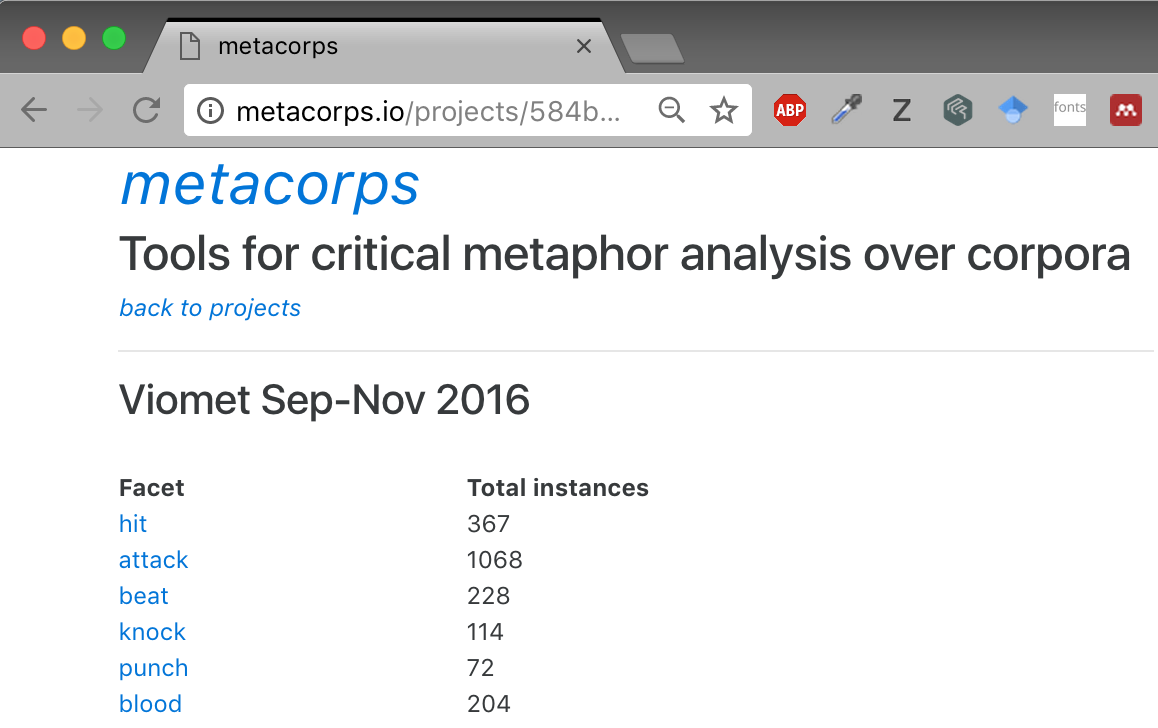
\includegraphics[width=\textwidth]{figures/facet-view.png}}
        \caption{Facet navigation}
    \end{subfigure}
    ~
    \begin{subfigure}[b]{0.45\textwidth}
            \frame{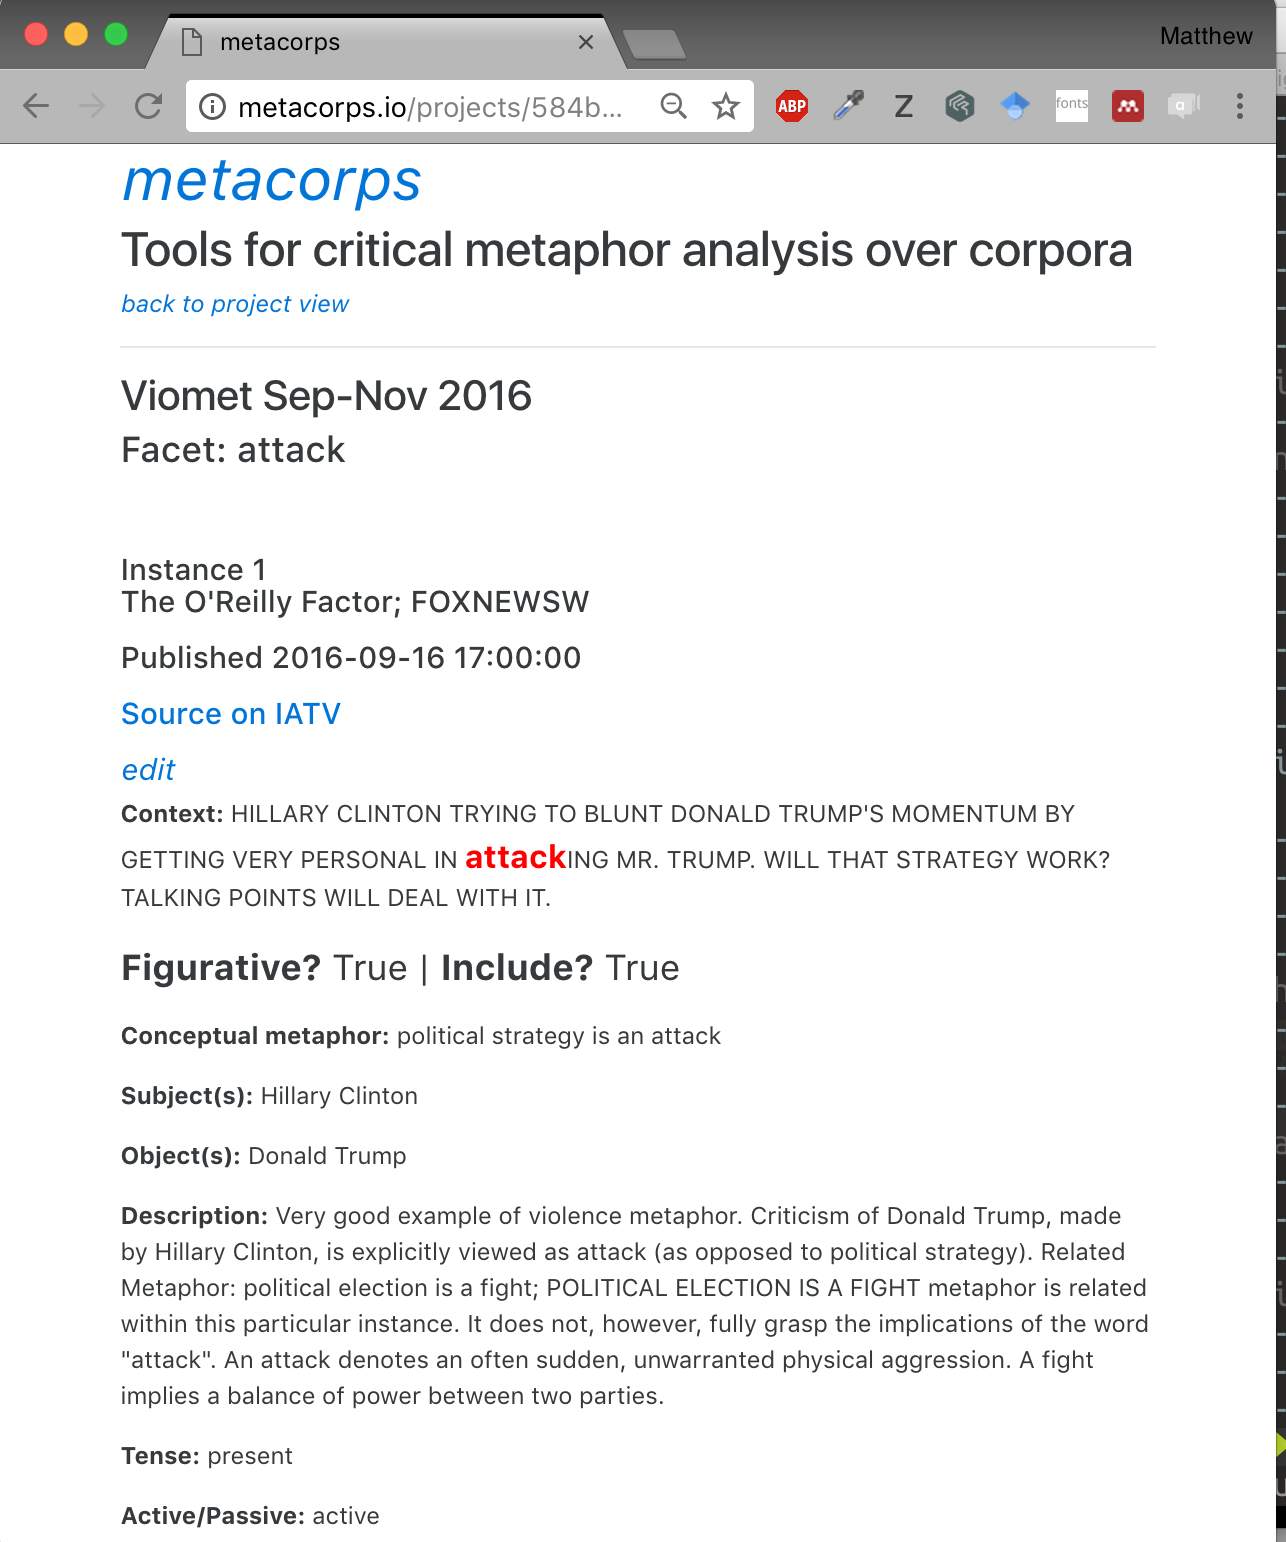
\includegraphics[width=\textwidth]{figures/instances-view.png}}
        \caption{Instance navigation for \textit{attack} facet}
    \end{subfigure}
    ~
    \caption{Screenshots of the Metacorps web app for metaphor annotation over
        corpora}
    \label{fig:metacorps-screenshots}
\end{figure*}

For this project, we had four people contributing to metaphor coding. In order
to keep track of progress and inform others of progress made, the Metacorps
web app includes a user log, shown in Figure \ref{fig:metacorps-home}. 
Once the coders finish annotating a project, it can be exported using an API
that's built-in to Metacorps itself. The user can export the annotations stored
in the database as CSV, or directly to a Pandas \texttt{DataFrame} object
\cite{McKinney2013} for interactive analysis or scripting.

\begin{figure}
    \centering
    \frame{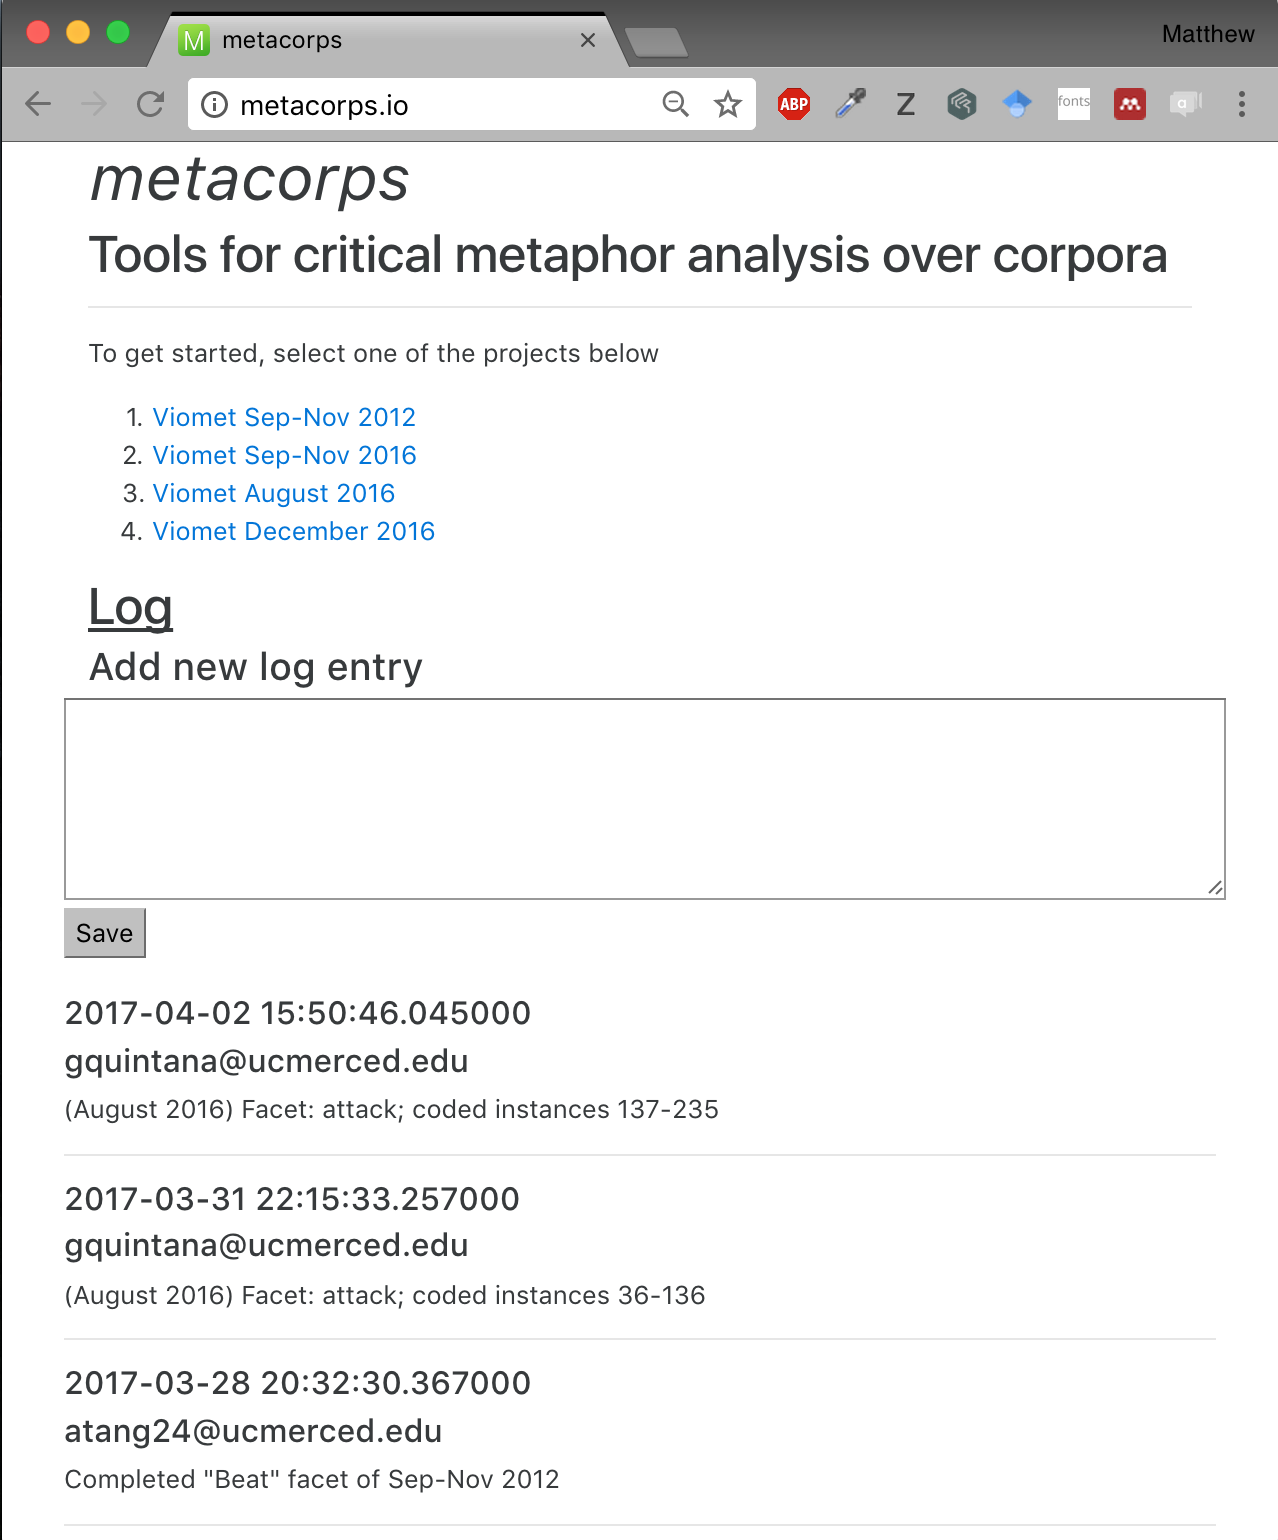
\includegraphics[width=0.75\textwidth]{figures/home-log.png}}
\caption{Home page of Metacorps web app. The metaphor coders use the log to
    inform others of progress. This is just the first step in making the
    app more social and collaborative.}
\label{fig:metacorps-home}
\end{figure}


